\subsection{Language}\label{Language}

At a syntactic level, Delta is a language with constructs for declaring formulas, interactive variables, semantics, connections, and steps (see Figure~\ref{fig:bnf-grammar} for a full BNF grammar). At a deeper conceptual level, Delta's language is a solution to three major concerns in making formulas interactive: \emph{substituting} instantiations in place of static expressions, supporting \emph{walkthroughs}, and \emph{synchronizing} between parts of a formula and other artifacts. We review the language as a tour of the constructs that addressed each concern.

\subsubsection{Substitution}
The language needs to let authors replace static mathematical expressions with more expressive and interactive variants. To this end, the language lets them select \textit{variables} from the formula according to their literal LaTeX and then specifying what is to take place with them. Variables can be \emph{labeled}. They can also be \emph{replaced}, where a concrete value is substituted in its place. When a value is shown, in label or in-situ, it can be configured to fixed \emph{precision} or \emph{significant digits}. A value can be made configurable through \emph{scrubbing} or \emph{direct entry}. For the former, bounds can be placed to constrain the space of exploration by setting \emph{defaults} and the \emph{range} and \emph{step size} of changes. Currently, values can be \emph{numbers} or \emph{lists}; the latter does not yet support interaction but can be displayed and used in semantics. Each of these aspects is configurable with a single property added to a variable's spec. The intent behind this decision was to make it \textbf{\textit{trivially possible to define and edit essential aspects of a variable's explanation}}.

Values come from the definition of the \emph{semantics}. Semantics are defined as JavaScript functions mapping input variables to output variables. To lower unnecessary barriers, authors do not have to explicitly mark variables as inputs or outputs; they just have to define interaction types on individual variables and provide a mapping in semantics. We opted for JavaScript semantics to enable \textbf{\textit{expressivity and familiarity in defining computation}}.

Delta provides a mechanism for \emph{graphical representations} of expressions. This is one form of augmentation from \citet{Head2022-ws}'s review that we believe hasn't been supported by prior toolkits. In Delta, an author can provide a user-defined JavaScript function that maps a variable's value to an SVG (e.g., clock hands rotating based on time); this is then substituted into the variable's position in the formula.

\subsubsection{Walkthroughs} The language lets an author describe a formula through series of \emph{steps}. In its current design, \textbf{\textit{Delta aligns explanation sequence with semantics}}. As we developed examples, we realized that sequential explanations required complex logic---for instance, in a summation, one might want to show example values, but only for the first few terms. Here, an imperative abstraction would have been useful; realizing there was already one available in the semantics function, we unified steps with semantics.

In Delta, a step is defined as breakpoint in the semantics; it is inserted alongside the computation code. Each call to \texttt{step} can define what should show at that step, including an optional global \emph{description} to appear above the full formula and \emph{labels} for individual variables and expressions. Selector syntax for variables and expressions is the same as in the variable spec. To split up labels one after another within the same computational stage, an author could simply sequence two step calls right after each other.

\subsubsection{Synchronization}\label{Synchronization}
Interactive formulas are often situated in larger math narratives, and the language provides a number of facilities to help plug formulas into those narratives.

For a formula to communicate with other artifacts, all artifacts must belong to the same React \emph{context provider} object from our components library. Then, different artifacts can refer to the same variables. For instance, an \textit{inline variable} can be added to a text that refers to a variable ID from a Delta spec. These two become linked (hovering over one highlights the other; either can be interacted with; the values change in tandem). Variables can be rendered as symbols or concrete values. \emph{Systems of formulas} are supported by using multiple formulas in the same context with shared variable names; again, changing one variable propagates to the other.

In many documents an author might wish to integrate formulas with bespoke visuals. In this case they can wrap their content in a ``\emph{custom}'' component, which has access to the \texttt{vars} object from semantics and therefore can read and write shared variable values.

Delta provides some support for generating the most basic kinds of linked visuals. As described in the scenario above, authors can define \emph{2D} ad \emph{3D graphs} that associate their \emph{axes} with variables. To populate these graphs, the author needs to \emph{sample} data points from a semantics function; in this way the semantics function serves to define the curves and surfaces. The \emph{interaction} property for an axis describes how drag actions on points can map to changes to variable values. Sample data is made accessible to outside artifacts through additional helper functions. Generated graphs are constrained to the \emph{ranges} of associated variables defined in the variables spec. Graph elements like points and vectors can synchronize with walkthroughs by referencing a \texttt{stepId}, an optional identifier authors assign when defining a step; by default, elements appear only for their associated step, but setting \texttt{persistence: true} causes them to accumulate across steps.

A philosophy behind our approach to synchronization is to, across contexts, leverage \textit{\textbf{variables names as universal indices into a shared store}}. These variable names are always snippets of the original LaTeX. They are used the same way regardless of calling context (variables spec, \texttt{vars} object, graph spec, external references). An example of leveraging this to interrelate multiple formulas, an inline variable, steps, and graphs is shown in Figure~\ref{fig:system}.

\begin{figure*}[t]
\centering
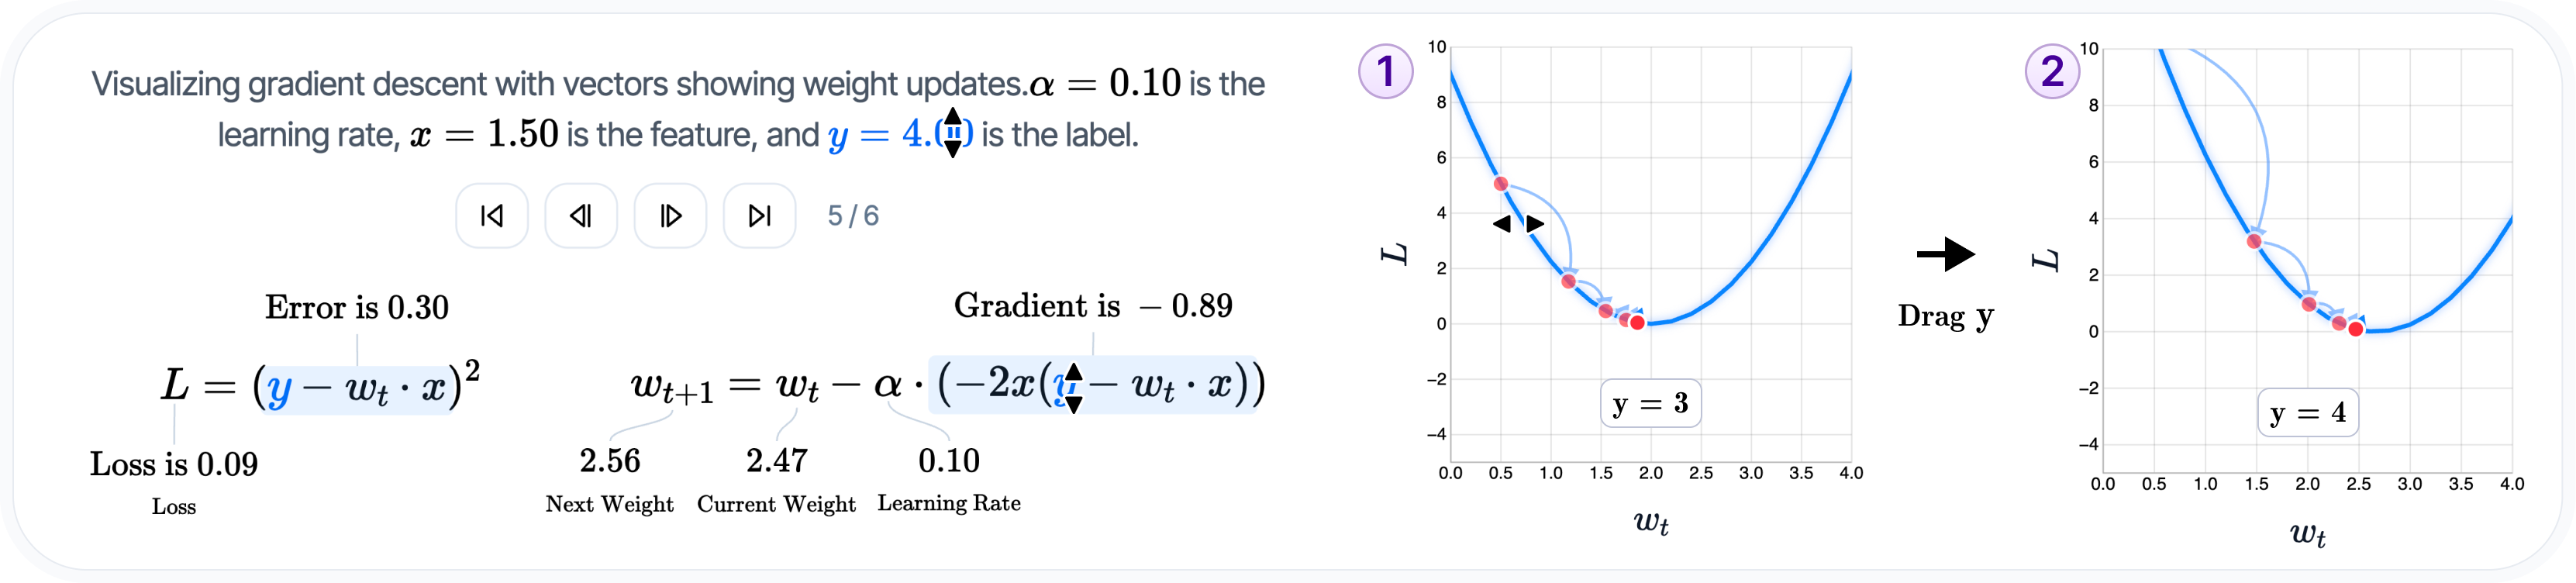
\includegraphics[width=\textwidth]{fig/system.png}
\caption{\textbf{Reactive propagation across steps and visualizations.} \textmd{Dragging $y$ in the prose, in the formula or on the graph's line (1) triggers re-execution of the semantics function, updating all intermediate step values and shifting the visualization vectors (2) to reflect the new loss landscape. See Figure~\ref{fig:gradient-config} for the full configuration. }}
\label{fig:system}
\end{figure*}

\subsection{Example Gallery}\label{Gallery}

Delta supports a broad array of interactive formulas across diverse contexts. We demonstrate this by reviewing examples we created to exercise the system, depicted in Figure~\ref{fig:teaser}. With each, we describe new design patterns and language constructs used.

\medskip

\emph{Kinetic Energy (1).} Our basic running example, where a formula serves as a calculator with variables as inputs controlled by scrubbing and direct editing. Uses \emph{formula}, \emph{variable specifications}, \emph{labels}, \emph{inline values}, \emph{drag} and \emph{scrub} interactions, \emph{precision}, and \emph{semantics}.

\emph{Probability Operations (2).} Two related formulas---$P(A \cap \neg B) = P(A) - P(A \cap B)$ and $P(B \cap \neg A) = P(B) - P(A \cap B)$---share a common synchronized variable $P(A \cap B)$. Scrubbing the intersection probability simultaneously updates both equations. Synchronization is coordinated by a \emph{shared variable ID} between formulas. 

\emph{Exponential Decay (3).} Dynamic visuals in the formula: glow of radiation signs and speed of clock ticking are influenced by current variable values. Uses parametric SVG \emph{graphical representations}.

\emph{Arithmetic Mean (4).} Our basic example walkthrough that shows accumulation of a sum in computing a mean. Uses \emph{steps}, which provide \emph{descriptions} and \emph{labels} for expressions at each step.

\emph{Linear Combination of Vectors (5).} Computation involving vectors, where scrubbing over scalar coefficients $k_1$ and $k_2$ immediately updates the result vector. Uses same constructs as (1).

\emph{Matrix Multiplication (6).} A $3 \times 3$ matrix product allows readers to scrub individual matrix entries and observe the updated values. Uses same constructs as (1), along with \emph{custom} external buttons (``Identity Matrix A,'' ``Reset All to Zero'') that provide meaningful ways to simultaneously set groups of variables.

\emph{Harmonic Motion (7).} The wave equation paired with a synchronized time-series plot. Dynamic iconic glyphs above each parameter---a stretched wave for amplitude, compressed oscillations for frequency, a phase-shifted curve for $\phi$---provide visual mnemonics. Dragging the point updates $t$ and dragging the curve updates the amplitude variable in the formula. Uses \emph{graphics} in \emph{labels} with linked \emph{2D graph} and \emph{interaction} controls mapping \emph{drags} to variable changes.

\emph{Gradient Descent (8).} Gradient descent is demonstrated with a linked loss function $L = (y - w_t \cdot x)^2$, weight update rule $w_{t+1} = w_t - \alpha \cdot (-2x(y - w_t \cdot x))$, and loss landscape visualization. As readers step through iterations, points and arrows accumulate on the graph tracing the optimization path. Dragging the learning rate $\alpha$ or target $y$ triggers re-execution of all steps, updating formula annotations and graph elements. Uses nearly all features. Semantics provide discrete \emph{steps} for the plot.

\medskip